\section{Arcs and Sectors}

\subsection{Arc: \texttt{\textbackslash tkzDrawArc}}

\subsubsection{Default behavior \texttt{towards}}

\begin{tkzexample}[latex=5cm,small]
  \begin{tikzpicture}[scale=1,>=Latex]
    \tkzDefPoints{0/0/O,2/-1/A,1/1/B}
    \tkzDrawArc[color=blue,->](O,A)(B)
    \tkzDrawArc[color=red,->](O,B)(A)
    \tkzDrawLines[add = 0 and .5](O,A O,B)
    \tkzDrawPoints[size=1.5pt](O,A,B)
    \tkzLabelPoints[below](O,A,B)
  \end{tikzpicture}
\end{tkzexample}

\subsubsection{Rotate}

\begin{tkzexample}[latex=5cm,small]
  \begin{tikzpicture}[scale=0.7]
    \tkzDefPoints{0/0/O,2/-2/A,3/0/C}
    \tkzDefPoint(60:2){B}
    \tkzDrawLines[add = 0 and .5](O,A O,B O,C)
    \tkzDrawArc[rotate,color=red](O,A)(180)
    \tkzDrawPoints[size=1.5pt](O,A,B)
    \tkzLabelPoints[below](O,A,B)
    \tkzMarkAngle[mark=none,size=0.5cm](C,O,B)
    \tkzLabelAngle[pos=1](C,O,B){$60\degree$}
    \tkzMarkAngle[mark=none,size=0.75cm](A,O,C)
    \tkzLabelAngle[pos=1.25](A,O,C){$45\degree$}
  \end{tikzpicture}
\end{tkzexample}

\subsubsection{Radius}

\begin{tkzexample}[latex=5cm,small]
  \begin{tikzpicture}[scale=.8]
    \tkzDefPoints{0/0/O,0/-3/x,3/0/y}
    \tkzDrawArc[R,color=orange,double](O,3cm)(270,360)
    \tkzDrawArc[R,color=blue,double](O,2cm)(0,270)
    \tkzDrawPoint(O)
    \tkzLabelPoint[above](O){$O$}
    \tkzDrawSegment[densely dotted](O,x)
    \tkzDrawSegment[densely dotted](O,y)
  \end{tikzpicture}
\end{tkzexample}

\subsubsection{\texttt{delta}}

\begin{tkzexample}[latex=5cm,small]
  \begin{tikzpicture}[scale=0.8]
    \tkzDefPoints{0/0/A,5/0/B}
    \tkzDefPointBy[rotation= center A angle 60](B)
    \tkzGetPoint{C}
    \tkzDefPointBy[rotation= center A angle -10](B)
    \tkzGetPoint{D}
    \tkzDrawArc[orange,delta=10](A,B)(C)
    \tkzDrawArc[orange,delta=10](B,C)(A)
    \tkzDrawPoints(A,B,C,D)
    \tkzLabelPoints(A,B,C,D)
    \tkzDrawSegments[color=gray,dashed](A,B A,D)
    \tkzMarkAngle[mark=none,size=1.5cm](D,A,B)
    \tkzLabelAngle[pos=2.5](D,A,B){$10\degree$}
  \end{tikzpicture}
\end{tkzexample}

\subsubsection{\texttt{angles}}

\begin{tkzexample}[latex=6cm,small]
  \begin{tikzpicture}[scale=.75]
    \tkzDefPoint(0,0){A}
    \tkzDefPoint(5,0){B}
    \tkzDefPoint(2.5,0){O}
    \tkzDefPointBy[rotation=center O angle 60](B)
    \tkzGetPoint{D}
    \tkzSetUpLine[color=Maroon]
    \tkzDrawArc[angles,color=orange](O,B)(30,120)
    \tkzDrawArc[angles,color=blue](B,O)(100,150)
    \tkzDrawLines(A,B O,D B,D)
    \tkzDrawPoints(A,B,O,D)
    \tkzLabelPoints(A,B,O,D)
  \end{tikzpicture}
\end{tkzexample}

\subsection{Sector: \texttt{\textbackslash tkzDrawSector}}

\begin{tkzexample}[latex=5cm,small]
  \begin{tikzpicture}[scale=1.5]
    \tkzDefPoint(0,0){O}
    \tkzDefPoint(2,2){A}
    \tkzDrawSector[rotate,draw=red!50!black,%
      fill=red!20](O,A)(30)
    \tkzDrawSector[rotate,draw=blue!50!black,%
      fill=blue!20](O,A)(-30)
  \end{tikzpicture}
\end{tkzexample}

\begin{tkzexample}[latex=6cm,small]
  \begin{tikzpicture}[scale=.67]
    \tkzDefPoint(0,0){O}
    \tkzDefPoint(-30:3){A}
    \tkzDefPointBy[rotation = center O angle -60](A)
    \tkzDrawSector[fill=red!50](O,A)(tkzPointResult)
    \begin{scope}[shift={(-60:1)}]
      \tkzDefPoint(0,0){O}
      \tkzDefPoint(-30:3){A}
      \tkzDefPointBy[rotation = center O angle -60](A)
      \tkzDrawSector[fill=blue!50](O,tkzPointResult)(A)
    \end{scope}
  \end{tikzpicture}
\end{tkzexample}

\subsection{Compass: \texttt{\textbackslash tkzCompass}}

\begin{tkzexample}[latex=5cm,small]
  \begin{tikzpicture}
    \tkzSetUpCompass[style={<->}]
    \tkzDefPoint(1,1){A}
    \tkzDefPoint(6,1){B}
    \tkzInterCC[R](A,4)(B,3)
    \tkzGetPoints{C}{D}
    \tkzDrawPoint[size=1.5pt](C)
    \tkzCompass[color=red,>=latex,length=1.8](A,C)
    \tkzCompass[color=blue,delta=30](B,C)
    \tkzDrawSegments(A,B A,C B,C)
  \end{tikzpicture}
\end{tkzexample}

\subsection{\texttt{\textbackslash tkzShowLine}}

\begin{tkzexample}[latex=6cm,small]
  \begin{tikzpicture}
    \tkzDefPoints{0/0/A, 3/2/B, 1.5/2.5/C}
    \tkzDefLine[perpendicular=through C,K=-.5](A,B)
    \tkzGetPoint{c}
    \tkzShowLine[thick,color=blue,%
      perpendicular=through C,K=-.5,gap=3](A,B)
    \tkzDefLine[parallel=through A](C,c)
    \tkzGetPoint{a}
    \tkzShowLine[thick,color=red,%
      parallel=through A](C,c)
    \tkzDefPointBy[projection=onto A--B](c)
    \tkzGetPoint{h}
    \tkzMarkRightAngle[fill=lightgray,size=.2](c,h,A)
    \tkzDrawLines[add=.5 and .5](A,B C,c A,a)
    \tkzDrawPoints[size=1.5pt](A,B,C,h,c)
  \end{tikzpicture}
\end{tkzexample}
